\documentclass[12pt]{article}
\usepackage[paper=letterpaper,margin=2cm]{geometry}
\usepackage{enumitem}
\usepackage{amsmath}
\usepackage{graphicx}
\usepackage{xcolor}
\usepackage{tabularray}
\usepackage{mathtools}

\graphicspath{ {./images/} }

\begin{document}

\begin{titlepage}
    \begin{center}
        \vspace*{1cm}

        \textbf{Redes de Computadores}
        \vspace{0.5cm}

        Resumo
        \vspace{1.5cm}

        \textbf{Rafael Rodrigues}
        \vfill
        LEIC \\
        Instituto Superior Técnico \\
        2022/2023
    \end{center}
\end{titlepage}

\tableofcontents

\newpage

\section{Introduction}

\subsection{What is a Protocol?}
A protocol defines the format and the order of messages exchanged between two or more communicating entities, as
well as the actions taken on the transmission and/or receipt of a message or other event.
\begin{itemize}
    \item Hardware-implemented Protocol → Controls the flow of bits on the 'wire' between the 2 network cards.
    \item Congestion-Control Protocol → Controls the rate at which packets are transmitted between sender and receiver.
    \item Router Protocol → Determines a packet's path from source to destination.
\end{itemize}

\subsection{Network Edge}

\subsection{Network Core}

\subsubsection{Packet Switching}

\begin{itemize}
    \item Comunicação dividida em pacotes, que partilham recursos com os restantes utilizadores.
    \item Cada um usa a largura de banda toda do canal. Recursos usados quando necessários.
    \item Não há alocação de canais.
\end{itemize}

\subsubsection{Circuit Switching}

\begin{itemize}
    \item Reserva largura de banda em todo o percurso, somo se ligasse cabos fisicamente.
    \item Precisa de setup, não há partilha de recursos.
    \item Garantias de performance. 
\end{itemize}

\subsubsection*{Packet Switching vs Circuit Switching}

Packet Switching é excelente para comunicação bursty, cujas necessidade de recursos varia com o tempo.

\subsection{Performance Metrics}

\subsection{Protocol Layers}

To provide structure to the design of network protocols, network designers organize them in layers. \\
Each layer provides its service by (1) performing certain actions within
that layer and by (2) using the services of the layer directly below it.
\vspace{0.5cm} \\
Advantage → Layering provides a structured way to discuss system components. \\
Disadvantage → One layer may duplicate lower-layer functionality. \\

\begin{tabular}{ | c | }
    \hline Application \\
    \hline Transport \\
    \hline Network \\
    \hline Link \\
    \hline Physical \\ 
    \hline
\end{tabular}

\newpage

\section{Application Layer}

The application layer is where network applications and their application-layer protocols reside. The Internet's application layer includes many protocols, such as the HTTP protocol (which provides for Web document request and transfer), SMTP (which provides for the transfer of e-mail messages), and FTP (which provides for the transfer of files between two end systems). We'll see that certain network functions, such as the translation of human-friendly names for Internet end systems like www.ietf.org to a 32-bit network address, are also done with the help of a specific application-layer protocol, namely, the domain name system (DNS). We'll see in Chapter 2 that it is very easy to create and deploy our own new application-layer protocols.
\vspace{0.5cm} \\
An application-layer protocol is distributed over multiple end systems, with the application in one end system using the protocol to exchange packets of information with the application in another end system. We'll refer to this packet of information at the application layer as a message.

\subsection{Principles of Network Applications}

\subsubsection{Network Application Architectures}

\begin{itemize}
    \item Client-Server Architecture:
        \begin{itemize}
            \item One host (server) to many hosts (clients).
            \item Clients do not directly communicate with each other.
            \item The server has a fixed, well-known IP address, meaning a client can always contact the server.
        \end{itemize}
    \item P2P Architecture:
        \begin{itemize}
            \item Scalable
            \item Hard to manage
        \end{itemize}
\end{itemize}

\subsubsection{Processes Communicating}

\subsection{The Web and HTTP (Port 80)}

\subsubsection{Overview of HTTP}

\subsubsection{Non-Persistent and Persistent Connections}

\subsubsection{HTTP Message Format}

\subsubsection{User-Client Interaction: Cookies}

Cookies permitem que o protocolo HTTP mantenha estado. São guardadas pelo utilizador. \\
O servidor envia cookies (cookie header) na resposta HTTP.

\subsubsection{Web Caching}

\subsubitem \textbf{The Conditional GET}

Quando é solicitado um objeto que o browser já tem guardado em cache, o browser envia um GET condicional ao servidor, para verificar que a cópia guardada em cache está atualizada. \par
O servidor responde, mas caso não tenha sido modificado, o objeto não é enviado de modo a poupar bandwidth e melhorar o desempenho.

\subsection{Electronic Mail in the Internet [Port 25]}

\subsubsection{SMTP}

\subsubsection{Comparison with HTTP}

\subsubsection{Mail Message Formats}

\subsubsection{Mail Access Protocols}

\subsection{Domain Name System (DNS) [Port 53]}

\begin{itemize}
    \item Associa nomes \textbf{(domínios)} a endereços IP.
    \item Base de dados distribuída por uma hierarquia de servidores de nomes \textbf{(name servers)}.
    \item Acedida através de um \textbf{resolver}.
    \item Utiliza maioritariamente o protocolo UDP, é usado TCP se a resposta for demasiado grande.
\end{itemize}

\subsubsection{DNS Records}

Resource Records (RR): (\textbf{name}, \textbf{value}, \textbf{type}, ttl) \\\\
The meaning of \textbf{name} and \textbf{value} depend on \textbf{type}:

\begin{itemize}[topsep=0pt, itemsep=0pt]
    \item \textbf{type} = A:
        \begin{itemize}[topsep=0pt, itemsep=0pt]
            \item \textbf{name}: hostname
            \item \textbf{value}: IP address of the hostname
        \end{itemize}
    \item \textbf{type} = NS:
        \begin{itemize}[topsep=0pt, itemsep=0pt]
            \item \textbf{name}: domain
            \item \textbf{value}: hostname of an authoritative DNS server knowing how to obtain IP address for the domain
        \end{itemize}
    \item \textbf{type} = CNAME:
        \begin{itemize}[topsep=0pt, itemsep=0pt]
            \item \textbf{name}: alias hostname
            \item \textbf{value}: canonical hostname (real name)
        \end{itemize}
    \item \textbf{type} = MX:
        \begin{itemize}[topsep=0pt, itemsep=0pt]
            \item \textbf{name}: alias hostname of a \textbf{mail server}
            \item \textbf{value}: canonical hostname (real name)
        \end{itemize}
\end{itemize}

\subsection{File Distribution}

Distribution Time → Time it takes to get a copy of a file with size $F$ to all $N$ peers.

\subsubsection{Client-Server Architecture}

In the client-server architecture, none of the peers aid in distributing the file:

\begin{itemize}
    \item The server must transmit one copy of the file to each of the $N$ peers. Thus, the server must transmit $N\cdot F$ bits. Since the server's upload rate is $u_s$, the time to distribute the time must be at least $\displaystyle\frac{N\cdot F}{u_s}$
    \item Let $d_{min}$ be the smallest download rate among the $N$ peers. The peer with the $d_{min}$ cannot obtain all $F$ bits of the file in less than $\displaystyle\frac{F}{d_{min}}$ seconds. Thus, this is the distribution time. 
\end{itemize}

\begin{center}
    $\displaystyle D_{client-server}=
    max\left\{\frac{N\cdot F}{u_s},\frac{F}{d_{min}}\right\}$
\end{center}

\subsubsection{P2P Architecture}

In the P2P architecture, when a peer receives some file data, it can use its own upload capacity to redistribute the data to other peers:

\begin{itemize}
    \item The server must transmit $F$ bits of the file at least once into its access link. Since the server's upload rate is $u_s$, the minimum distribution time is at least $\displaystyle\frac{N\cdot F}{u_s}$
    \item Let $d_{min}$ be the smallest download rate among the $N$ peers. The peer with the $d_{min}$ cannot obtain all $F$ bits of the file in less than $\displaystyle\frac{F}{d_{min}}$ seconds. Thus, this is the distribution time.
    \item The total upload capacity of the system as a whole is equal to $u_{total} = u_s + u_1 + u_2+...+u_N$. The system must upload $F$ bits to each of the $N$ peers, thus delivering a total of $N\cdot F$ bits. This cannot be done at a rate faster than $u_{total}$. Hence, the minimum distribution time is also at least
    $\displaystyle\frac{N\cdot F}{u_{total}}$
\end{itemize}

\begin{center}
    $\displaystyle D_{client-server}=
    max\left\{\frac{F}{u_s},\frac{F}{d_{min}},\frac{N\cdot F}{u_{total}}\right\}$
\end{center}

\subsection{Socket Programming}

\subsubsection*{UDP}

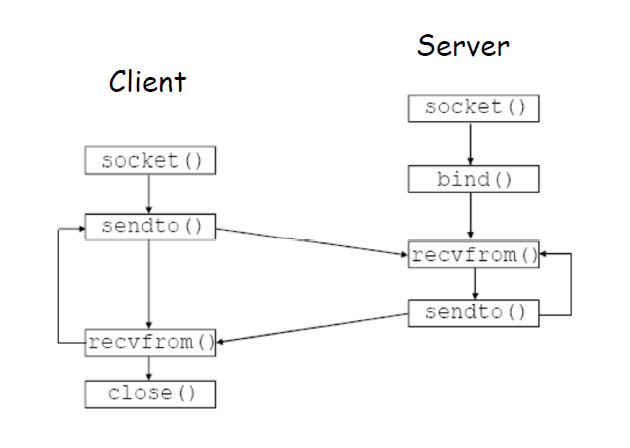
\includegraphics[scale=0.7]{UDP}

\subsubsection*{TCP}

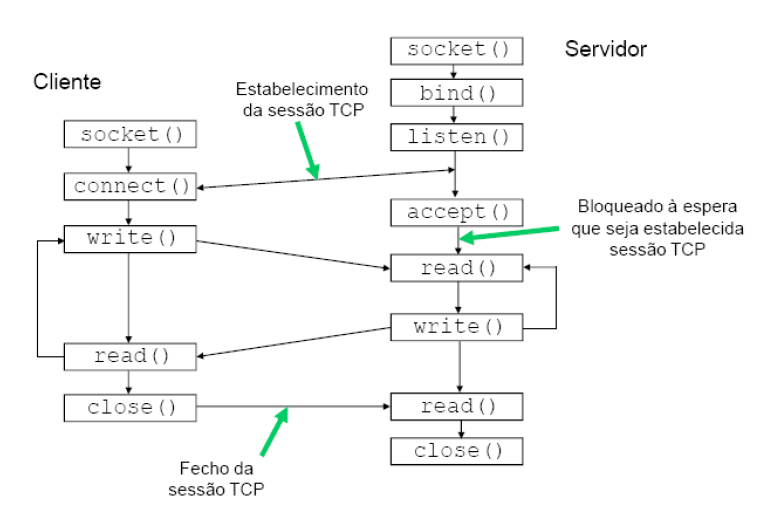
\includegraphics[width=\textwidth]{TCP}

\subsubsection*{TCP vs UDP}

\begin{tabular}{ p{3in} | p{3in} }
    TCP & UDP \\\hline
    read() and write() & sendto() and recvfrom() \\\hline
    Byte stream (no byte is lost) & Messages may be lost \\\hline
    Bytes read with read() may correspond to several write() & Preserves boundary between messages \\\hline
    Bytes written with write() may need to be read with several read() & Each message read with recvfrom() correspond to a single sendto() \\
\end{tabular}

\newpage

\section{Transport Layer}

The Internet's transport layer transports application-layer messages between application endpoints. In the Internet there are two transport protocols, TCP and UDP, either of which can transport application layer messages. TCP provides a connection-oriented service to its applications. This service includes guaranteed delivery of application-layer messages to the destination and flow control (that is, sender/receiver speed matching). TCP also breaks long messages into shorter segments and provides a congestion-control mechanism, so that a source throttles its transmission rate when the network is congested. The UDP protocol provides a connectionless service to its applications. This is a no-frills service that provides no reliability, no flow control, and no congestion control. In this book, we'll refer to a transport-layer packet as a segment.

\subsection{User Datagram Protocol (UDP)}

\begin{itemize}
    \item Um socket UDP é identificado pelo tuplo: (dest IP, dest port)
    \item Quando recebe datagrama UDP, entrega ao socket com esse IP:porto
    \item Sem ligações nem garantias de ordem ou entrega
    \item Sem controlo de congestão
    \item Checksum (opcional): %TODO
\end{itemize}

Headers pequenos, é simples e rápido. Usado para streaming, DNS e SNMP.

\subsection{Transmission Control Protocol (TCP)}

\begin{itemize}
    \item Um socket TCP é identificado pelo tuplo: (src IP, src port, dest IP, dest port)
    \item Há 1 socket por ligação (cliente), cada uma abre um socket novo.
    \item Entrega fiável e ordenada.
    \item 
\end{itemize}

\newpage

\section{Network Layer}

The Internet's network layer is responsible for moving network-layer packets known as datagrams from one host to another. The Internet transport-layer protocol (TCP or UDP) in a source host passes a transport-layer segment and a destination address to the network layer, just as you would give the postal service a letter with a destination address. The network layer then provides the service of delivering the segment to the transport layer in the destination host. 
\vspace{0.5cm} \\
The Internet's network layer includes the celebrated IP protocol, which defines the fields in the datagram as well as how the end systems and routers act on these fields. There is only one IP protocol, and all Internet components that have a network layer must run the IP protocol. The Internet's network layer also contains routing protocols that determine the routes that datagrams take between sources and destinations. The Internet has many routing protocols. As we saw in Section 1.3, the Internet is a network of networks, and within a network, the network administrator can run any routing protocol desired. Although the network layer contains both the IP protocol and numerous routing protocols, it is often simply referred to as the IP layer, reflecting the fact that IP is the glue that binds the Internet together.

\subsection{Overview of Network Layer}

The primary role of the \textbf{data plane} is to forward datagrams from its input links to its output links. 
\vspace{0.5cm} \\
The primary role of the \textbf{control plane} is to coordinate these local, per-route forwarding actions so that datagrams are ultimately transferred end-to-end, along paths of routers between source and destination.

\subsubsection{Forwarding and Routing: The Data and Control Planes}

The primary role of the network layer is to move packets from the sending host to a receiving host. Thus, there are 2 important network-layer function:

\begin{enumerate}
    \item Forwarding → When a packet arrives at a router's input link, it must move the packet to the appropriate output link. A packet might also be blocked from exiting a router or duplicated and sent over multiple outgoing links. \\
    \textbf{Forwarding is router-local}, and is the key function performed by the data-plane functionality.
    \item Routing → The network layer must determine the path taken by packets as they flow from a sender to a receiver. To do so, the network layer uses multiple routing algorithms. Routing refers to the network-wide.
    \textbf{Routing is a network-wide process}.
\end{enumerate}

\subsection{}

\subsection{The Internet Protocol (IP)}

\subsubsection{Fragmentation}

\subsubsection{Adressing}

\subsubsection*{Dynamic Host Configuration Protocol (DHCP) [Server Port 67, Client Port 68]}

\begin{itemize}
    \item Mensagens de DHCP são em UDP.
    \item Endereços são emprestados por um tempo finito (lease time).
    \item Após 50\% do lease time, o cliente tenta renovar o IP (\textbf{DHCP Request}). \\
        Se não conseguir, tenta de novo a 85\%.
\end{itemize}

Outras mensagens:

\begin{itemize}[topsep=0pt, itemsep=0pt]
    \item Decline: cliente rejeita oferta
    \item NACK: servidor não consegue satisfazer pedido
    \item Release: cliente informa que já não quer usar endereço
    \item Inform: cliente pede parâmetros extra
\end{itemize}

\subsubsection*{Network Address Translation (NAT)}

\begin{enumerate}
    \item Quando um utilizador da rede privada envia um pacote, o NAT substitui o endereço IP interno do remetente pelo externo, e memoriza o correspondente.
    \item Quando recebe uma resposta o NAT restaura o IP interno.
\end{enumerate}

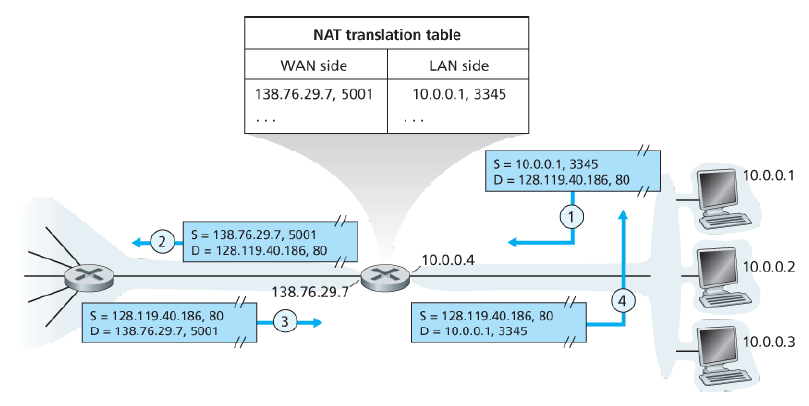
\includegraphics[width=0.9\textwidth]{NAT}

\subsection{Software Defined Network (SDN)}

A abordagem usando SDN para a implementação da camada de rede considera que apenas o plano de dados (\textbf{Data Plane}) é implementado em cada encaminhador.

\newpage

\section{Link Layer}

The Internet's network layer routes a datagram through a series of routers between the source and destination. To move a packet from one node (host or router) to the next node in the route, the network layer relies on the services of the link layer. In particular, at each node, the network layer passes the datagram down to the link layer, which delivers the datagram to the next node along the route. At this next node, the link layer passes the datagram up to the network layer. 
\vspace{0.5cm} \\
The services provided by the link layer depend on the specific link-layer protocol that is employed over the link. For example, some link-layer protocols provide reliable delivery, from transmitting node, over one link, to receiving node. Note that this reliable delivery service is different from the reliable delivery service of TCP, which provides reliable delivery from one end system to another. Examples of link-layer protocols include Ethernet, WiFi, and the cable access network's DOCSIS protocol. As datagrams typically need to traverse several links to travel from source to destination, a datagram may be handled by different link-layer protocols at different links along its route. For example, a datagram may be handled by Ethernet on one link and by PPP on the next link. The network layer will receive a different service from each of the different link-layer protocols. In this book, we'll refer to the link-layer packets as
frames.

\subsection{}

\subsection{Error Detection and Correction Techniques}

\subsubsection{Parity Checks}

\subsubsection{Cyclic Redundancy Check (CRC)}

\subsection{Multiple Access Links and Protocols}

\subsubsection{Channel Partitioning Protocols}

\subsubsection{Random Access Protocols}

\subsubsection{Dynamic Allocation Protocols (Taking-Turns)}

\subsection*{Summary of MAC Protocols}

\begin{tabular}{ | c | c | c | }
    \hline
    & Dynamic Allocation & Random Access \\ \hline
    High Loads & Efficient & Collision overhead \\ \hline
    Low  Loads & Active nodes have to wait for idle nodes & Efficient \\ \hline
\end{tabular}

\subsection{Switched Local Area Networks}

\subsubsection{Link-Layer Addressing and ARP}

\subsubsection*{MAC Addresses}

\subsubsection*{Address Resolution Protocol (ARP)}

\subsubsection{Ethernet}

\subsubsection{Link-Layer Switches}

\subsubsection*{}

\subsubsection*{Self-Learning}

Switches are self-learning, meaning the switch table is built automatically, dynamically and autonomously.

\begin{enumerate}
    \item The switch table is initially empty.
    \item For each incoming frame received on an interface, the switch stores in its table: \\
        \begin{tabular}[t]{ | c | c | c | }
            \hline
            MAC Address & Interface & Current time \\\hline
            E6-E9-00-17-BB-4B & 1 & 00:01 \\\hline
        \end{tabular}
    \item The switch deletes an address in the table if no frames are received with that address as the source address after some time (\textbf{aging time}).
\end{enumerate}

\subsubsection*{Spanning-Tree Protocol (STP)}

\begin{itemize}
    \item Establishes a root node called the root bridge.
    \item Constructs a topology that has one path from/to every network node.
    \item Resulting tree originates from the root bridge.
    \item Redundant links that are not part of the shortest path are blocked.
\end{itemize}

\subsubsection*{Bridge Protocol Data Unit (BPDU)}

Convention for Conf-BPDUs: Root ID . Root Path Cost . Bridge ID \\\newline
A configuration $C_1$ is said to be better than $C_2$ if (ordered by decreasing importance):

\begin{enumerate}[topsep=0pt, itemsep=0pt]
    \item $C_1$ Root ID is lower than that of $C_2$.
    \item $C_1$ Root Path Cost is lower than that of $C_2$.
    \item $C_1$ Bridge ID is lower than that of $C_2$.
    \item $C_1$ Port ID is lower than that of $C_2$.
\end{enumerate}

\subsubsection{Virtual Local Area Networks (VLANs)}

\newpage

\section{Wireless and Mobile Networks}

\subsection{WiFi [802.11]}

\subsubsection{Architecture}



\subsubsection{MAC Protocol}

\subsubsection*{Multiple Access}

\subsubsection*{Collision Avoidance}

\end{document}
